\section{Solving the prisonersdilemma}
One possibility for solving the problem that arised in the last section is to introduce a leader follower game. In this game the players does not act at the same time, but in order, and they can observe the other players action.
If we consider a game with only two players, player one are the first to select an action. He chooses to insure or not. Then after observing this action player two chooses if he would like to insure or not. Then they choose if they would establish link or not, in the same order.
The stackelberg model or the leader follower game, can be solved to find the subgame perfect Nash equilibrium. This is a strategy profile where every player plays his best response to the other players strategies. 


In this type of game the leader, will benefit from a first mover advantage, because he can now force the game in a direction he prefers. 
\begin{equation}
I_{l}<\beta \text{ and } I_{l}>\beta-r \text{ and } r<\beta
\label{eq:stackelbergcondition}
\end{equation}
By finding all subgame equilibria in Figure \ref{fig:stackelberg} except the last one, i.e. the subgame where player one chooses to Insure or not, we get this subgame equilibria: $(L,\overline{L^{I}_{1}},\overline{L^{II}_{1}},L^{III}_{1}), (I_{2},\overline{I^{I}_{2}},L_{2}L^{I}_{2},\overline{L^{II}_{2}},L^{III}_{2})$
We have now analyzed the different outcomes of player 1 choosing insure or not, thus he can now see what is the best thing for him to do. The two options he can choose between are: Insure and get payoff $\beta-I_{l}$ or not insure and get payoff $\beta-r$. I.e. if $I_{l}<r$ player one will chose to insure, and thus forcing the game to end up in a equilibrium where both players insure and establish link. If the cost of insuring is higher than the expected risk cost $r$, then obviously there is no reason to choose insurance.
From this we see that if the insurance price are set to the right amount, one player can force the outcome of the game to be the socially optimal outcome. 

Solve prisoners dilemma problem by forcing the other one to choose insurance


\begin{figure}[h]
\centering
  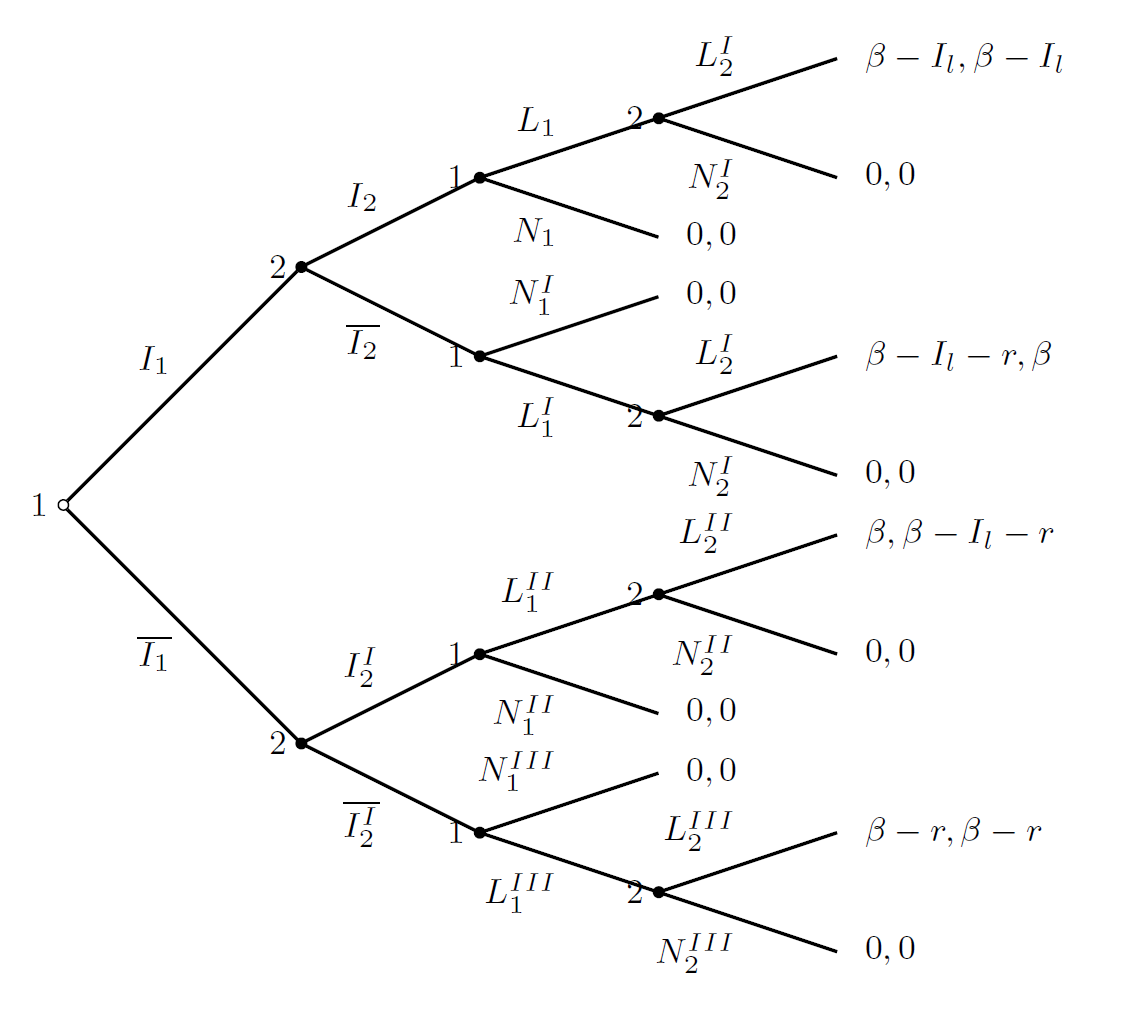
\includegraphics[width=0.9\linewidth]{../Figures/stackelberggame.png}
  \caption{\label{fig:stackelberg} Leader follower game, first player 1 chooses to insure or not, then player 2, and then they choose to establish link or not in the same order.}
\end{figure}
